\section{Embedded Systems}
\label{sec:EmbeddedSystems}
Ein Embedded System oder auf Deutsch ein eingebettetes System, wird als eine integrierte,
mikroelektronische Steuerung angesehen, welches meist darauf ausgelegt ist eine spezifische Aufgabe
zu erledigen. Dabei setzt sich ein eingebettetes System auch aus dem Zusammenspiel zwischen
Hardware und Software zusammen. Solche eingebetteten Systeme haben meist kein ausgeprägtes
Benutzerinterface und können weitergehend in die zwei unterklassen, Open und Deeply Embedded
Systems unterteilt werden.
\begin{figure}[h]
    \centering
    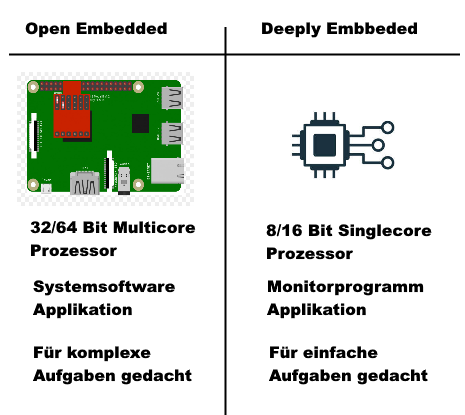
\includegraphics[width=0.55\textwidth, center]{StandDerTechnik/OpenDeeplyEmbeddedNew}
    \caption[Open vs Deeply Embedded Systeme]{Open vs Deeply Embedded Systeme
    \cite{EmbeddedLinuxQuade}[vgl.]}
    \label{img:OpenDeeplyEmbedded}
\end{figure}

Neben der logischen Korrektheit die eingebettete Systeme an den Tag legen müssen, lassen sie sich
durch eine Reihe unterschiedlicher Anforderungen und eigenschaften von den heutzutage üblichen
Anwedendungen abgrenzen. Unter anderem wird bei eingebettete Systeme ein sogenanntes
\emph{Instant on} gefordert, welches besagt, dass das Gerät unmittelbar nach dem Einschalten
betriebsbereit sein muss \cite{EmbeddedLinuxQuade}[vgl.].
\newline
\newline
Weitere Anforderungen die bei Embedded Systemen zustande kommen, sind in der Folgenden Tabelle
abgebildet:

\begin{table}[ht]
    \centering
    \begin{tabularx}{\textwidth}{md}
        \textbf{Anforderung}     & \textbf{Beschreibung} 	\\ \hline
        Funktionalität 			& Die Software muss schnell und korrekt sein	\\\rowcolor{Gray}
        Preis 				    & Die Hardware darf nicht zu kostenspielig sein				\\
        Robustheit				& Muss auch in einem rauen Umfeld funktionieren				\\\rowcolor{Gray}
        Fast poweroff			& Muss in der Lage sein schnell das komplette System Abzuschalten \\
        Räumliche Ausmaße		& Muss klein sein, um sich in ein System einbinden zu können	\\\rowcolor{Gray}
        Nonstop-Betrieb			& Muss in der Lage sein, im Dauerbetrieb laufen zu können	\\
        Lange Lebensdauer		& Muss in der Lage sein, mehr als 30 Jahre zu laufen ohne groß zu
        verschlechtern
    \end{tabularx}
    \caption{Anforderungen an eingebettete Systeme \cite{EmbeddedLinuxQuade}}
    \label{table:AnforderungenEingebetteteSysteme}
\end{table}

\subsection{Hardware}
\label{subsec:EmbeddedHardware}
Test
\subsection{Software}
\label{subsec:EmbeddedSoftware}
Genauso wie sich Embedded Systems in zwei Bereiche unterscheiden lassen können, kann die
Software eines Embedded System in Systemsoftware und funktionsbestimmende
Anwendungssoftware unterteilt werden.
Für ein \emph{Deeply Embedded System} wird in den meisten fällen ein Echtzeitbetriebssystem
(Realtime Operating System - RTOS) verwendet, welches an die Hardware angepasst ist.
\newline
\newline
Ganz anders sieht es im \emph{Non-Deeply Embedded Systems} Bereich aus. Da diese für sehr
komplexe Aufgaben zum Einsatz kommen, kommt es nicht selten
vor, dass eine \ac{gui} für ein solches System vonnöten ist. Deswegen basiert ein
\emph{Non-Deeply
Embedded Systems} auf einer Systemsoftware, die Programmierer*innen mehr Möglichkeiten bei
der Entwicklung geben. Unter anderem ist die Möglichkeit gegeben, die Programmiersprache
und
das \ac{gui}-Framework selbst auszusuchen \cite{EmbeddedLinuxQuade}[vgl.].
